\documentclass[11pt,letterpaper]{article}
\usepackage[T1]{fontenc}
\usepackage[utf8]{inputenc}
\usepackage{lmodern}
\usepackage[margin=0.85in]{geometry}
\usepackage{amsmath,amssymb}
\usepackage{graphicx,booktabs,array}
\usepackage{xcolor}
\usepackage{float,caption}
\usepackage{fancyhdr}
\usepackage{listings}
\usepackage{hyperref}
\definecolor{navy}{HTML}{183B56}
\definecolor{teal}{HTML}{116466}
\definecolor{codegray}{HTML}{F5F7F9}
\hypersetup{colorlinks=true,linkcolor=navy,urlcolor=teal,citecolor=navy,
  pdftitle={FRE7241 Homework 2: Volatility Timing and Hampel Strategies},
  pdfauthor={Panagiotis Housos}}
\pagestyle{fancy}
\fancyhf{}
\fancyhead[L]{\small FRE7241 \quad Homework 2}
\fancyhead[R]{\small Panagiotis Housos}
\fancyfoot[C]{\thepage}
\setlength{\headheight}{14pt}
\setlength{\parindent}{0pt}
\setlength{\parskip}{0.55em}
\setlength{\emergencystretch}{2em}
\clubpenalty=10000
\widowpenalty=10000
\renewcommand{\arraystretch}{1.12}
\captionsetup{font=small,labelfont=bf}
\lstdefinestyle{rcode}{language=R,basicstyle=\ttfamily\scriptsize,
  keywordstyle=\color{navy},commentstyle=\color{teal},
  stringstyle=\color{black},numbers=left,numberstyle=\tiny\color{gray},
  numbersep=7pt,backgroundcolor=\color{codegray},frame=single,
  rulecolor=\color{gray!25},breaklines=true,breakatwhitespace=false,
  columns=fullflexible,keepspaces=true,showstringspaces=false,
  tabsize=2,xleftmargin=12pt,framexleftmargin=10pt}
\lstset{style=rcode}
\newcommand{\wideinput}[3]{%
  \begin{table}[H]\centering
  \caption{#2}\label{#3}
  \resizebox{\linewidth}{!}{\input{tables/#1}}
  \end{table}}
\newcommand{\smallinput}[3]{%
  \begin{table}[H]\centering
  \caption{#2}\label{#3}
  {\small\input{tables/#1}}
  \end{table}}
\newcommand{\HWBestLambda}{0.3}
\newcommand{\HWBestSharpe}{0.6833}
\newcommand{\HWVolSharpe}{0.6548}
\newcommand{\HWSpySharpe}{0.5360}
\newcommand{\HWVolSortino}{0.7982}
\newcommand{\HWSpySortino}{0.6689}
\newcommand{\HWEligibleStocks}{717}
\newcommand{\HWMatchedStocks}{645}
\newcommand{\HWPersistenceCorrelation}{0.0293}
\newcommand{\HWPersistenceSlope}{0.0329}
\newcommand{\HWPersistencePValue}{0.4572}
\newcommand{\HWPersistenceRSquared}{0.000860}
\newcommand{\HWAllFullSharpe}{0.5415}
\newcommand{\HWAllOOSSharpe}{0.3866}
\newcommand{\HWTopFullSharpe}{1.3852}
\newcommand{\HWTopISSharpe}{2.1925}
\newcommand{\HWTopOOSSharpe}{0.4027}
\newcommand{\HWNxpiSharpe}{0.4509}
\newcommand{\HWNxpiHampelSharpe}{0.6674}
\newcommand{\HWVolScale}{0.003530}
\newcommand{\HWMinAvailable}{542}
\newcommand{\HWMaxAvailable}{655}


\begin{document}
\hypersetup{pageanchor=false}
\begin{titlepage}
\vspace*{0.6in}
{\color{teal}\large NYU Tandon School of Engineering\par}
\vspace{0.25in}
{\color{navy}\LARGE Algorithmic Portfolio Management\par}
\vspace{0.15in}
{\large FRE7241 \quad Homework 2\par}
\vspace{0.65in}
{\color{navy}\Huge Volatility Timing\\[0.12in]and Hampel Strategies\par}
\vspace{0.3in}
{\Large Methods, results, and interpretation\par}
\vspace{0.65in}
{\Large Panagiotis Housos\par}
\vspace{0.12in}
{\large November 7, 2026\par}
\vspace{0.3in}
{\small\url{https://github.com/ph2606/fre7241-homework-02}\par}
\end{titlepage}
\pagenumbering{roman}
\hypersetup{pageanchor=true}

\section*{Abstract}
This assignment evaluates two rules using the supplied course data. Part I
holds a position in SPY proportional to the inverse of its trailing
exponentially weighted volatility, delays the position by one trading day,
and deducts spread costs. A parallel parameter sweep compares nine decay
factors. Part II applies a three-observation Hampel mean-reversion rule to
individual stocks, averages their daily strategy PnLs, and examines the
relationship between Sharpe ratios through 2016 and from 2017 onward. The
top-100 portfolio is selected using the first period only. All curves show
cumulative sums of daily PnLs. Across \HWMatchedStocks{} stocks observed
in both intervals, the Sharpe correlation is
\HWPersistenceCorrelation{}, providing little evidence of persistence.
The top-100 portfolio's Sharpe declines from \HWTopISSharpe{} in sample to
\HWTopOOSSharpe{} afterward. The numerical results use frozen local data,
whose dates and universe differ from the template's illustrative outputs.

\tableofcontents
\clearpage
\pagenumbering{arabic}

\section{Data, conventions, and reproducibility}
\label{sec:data}
The completed submission is \texttt{Panagiotis\_Housos\_hw2.R}. The methods
follow the course's volatility and Hampel examples~\cite{univariate,app}.
The accompanying repository supplies the data snapshot, numerical outputs,
interactive plots, LaTeX source, and independent verification records:
\begin{center}
\url{https://github.com/ph2606/fre7241-homework-02}
\end{center}

Part I uses the installed \texttt{rutils::etfenv\$returns} SPY series after
removing missing returns: 8,352 daily observations from February 1, 1993
through April 7, 2026. Part II uses the supplied
\texttt{06\_Data/R\_Data/sp500\_prices.RData}, restricted to dates in
\texttt{"2006/"}. Its price matrix has 5,042 rows and 717 stock columns,
ending January 16, 2026. The portable input snapshot is
\texttt{data/hw2\_inputs.rds}.

The professor's template illustrates a different data version: 8,298 SPY
returns ending May 8, 2026, and approximately 1,000 stock strategies over
5,119 dates. These reference values are retained in the original template;
the completed code reports the values calculated from the available inputs.
Different dates, price revisions, and stock coverage can change every
performance statistic and ranking. The reference figures establish the
requested plot types.

The supplied SPY returns are daily log returns. Part II computes differences
of log prices. Returns and PnLs are kept as decimal values, and
\texttt{cumsum()} produces the plotted cumulative PnL. These sums are not
compounded dollar wealth. The backtests assume zero risk-free return,
252 trading days per year, and one-observation position delays. The
volatility estimator has the initialization exception documented below.

The course package version installed here exposes
\texttt{HighFreq::run\_var(timeser, lambdaf)}. The code passes the decay
parameter positionally; the template's \texttt{lambda} spelling also
matches the installed formal argument by R's partial-name matching.
Package versions, input hashes, and session
information are recorded under \texttt{reproducibility/}. This makes the
analysis repeatable without the instructor's absolute data path.

\section{Part I: inverse-volatility timing of SPY}
\subsection{I.1: positions, transaction costs, and risk adjustment}
Let $r_t$ denote SPY's daily log return. The course function
\texttt{HighFreq::run\_var()} calculates a trailing exponentially weighted
mean and variance. For the initial calculation the decay factor is
$\lambda=0.5$. Following the installed implementation, its recursion after
startup is
\begin{align}
\widehat\mu_t&=\lambda\widehat\mu_{t-1}+(1-\lambda)r_t,\\
\widehat v_t&=\lambda^2\widehat v_{t-1}
 +(1-\lambda^2)(r_t-\widehat\mu_t)^2.
\end{align}
The volatility estimate is the square root of the function's second output
column:
\begin{equation}
\widehat\sigma_t=\sqrt{\widehat v_t},\qquad
u_t=\frac{1}{\widehat\sigma_t},\qquad
w_t=u_{t-1},\quad w_1=0.
\label{eq:volposition}
\end{equation}
The one-day delay uses \texttt{rutils::lagit()}. The installed package
initializes its first variance from the first \emph{two} returns,
$\widehat v_1=(r_2-r_1)^2$. Consequently, the second observation's held
position uses its own return through this startup estimate. The assignment's
estimator and reference position convention are retained, so the second
observation is not fully ex ante. After this initialization, the delayed
recursive estimates use information available before the return to which
the position is applied.

The inverse-volatility position increases after quiet periods and decreases
after volatile periods. Its raw numerical size reflects reciprocal daily
volatility; the final PnLs are rescaled below.

The assigned bid--ask spread is $b=0.0001$. Trading at half the spread for
each unit of position turnover gives
\begin{equation}
c_t=\frac{b}{2}|w_t-w_{t-1}|,\qquad
q_t=w_t r_t-c_t,
\label{eq:costs}
\end{equation}
with zero initial position and the course's zero-padded difference
convention. A larger change in exposure incurs a larger cost. The net
strategy is then matched to SPY's observed daily standard deviation:
\begin{equation}
a=\frac{s(r)}{s(q)},\qquad p_t=a q_t.
\label{eq:scale}
\end{equation}
The scalar $a$ multiplies both trading gains and deducted costs. Since $a$
uses the full sample, the volatility matching is a descriptive comparison.
A trading implementation would estimate its scale from information already
available at the time. A positive constant scale leaves the Sharpe and
course-defined Sortino ratios unchanged.

The annualized Sharpe ratio is
\begin{equation}
\widehat{\mathrm{SR}}(x)=\sqrt{252}\,
\frac{\overline x}{s(x)}.
\label{eq:sharpe}
\end{equation}
The assignment's ratios use \texttt{rutils::calc\_sharpe()}, whose second row
uses the standard deviation of the subset of negative observations:
\begin{equation}
\widehat{\mathrm{Sortino}}_{\mathrm{course}}(x)
=\sqrt{252}\,\frac{\overline x}{s(\{x_t:x_t<0\})}.
\label{eq:sortino}
\end{equation}
This conditional downside standard deviation differs from downside
semideviation computed across every date. The report uses the course
definition consistently.

\wideinput{vol_metrics.tex}{SPY and the $\lambda=0.5$ volatility-timing
strategy. The strategy includes spread costs and is scaled to SPY's daily
standard deviation. Annualization uses 252 trading days.}{tab:volmetrics}

\begin{figure}[H]\centering
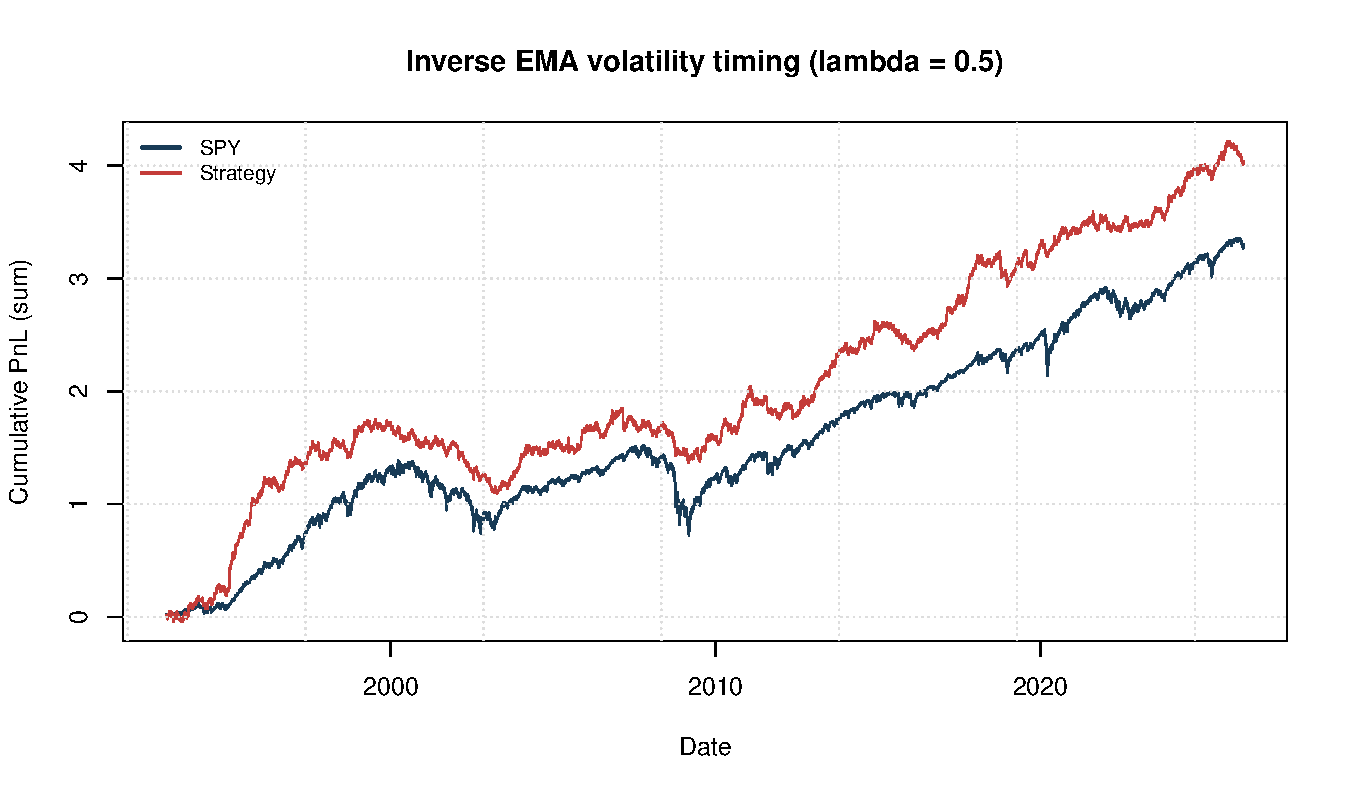
\includegraphics[width=0.94\linewidth]{figures/strat_voltiming_ema.pdf}
\caption{SPY and volatility-timing cumulative PnLs. The red strategy curve
includes the spread costs in Equation~\ref{eq:costs}; both series have the
same full-sample daily standard deviation.}
\label{fig:voltiming}
\end{figure}

Table~\ref{tab:volmetrics} compares average return relative to total and
negative-return variation. At $\lambda=0.5$, the net strategy Sharpe is
\HWVolSharpe{}, compared with \HWSpySharpe{} for SPY. The corresponding
course Sortino ratios are \HWVolSortino{} and \HWSpySortino{}.
Figure~\ref{fig:voltiming} also shows the timing
of gains and losses; its terminal height alone is not a risk-adjusted
performance measure. The rule can remain exposed when volatility rises
abruptly because yesterday's estimate determines today's position. The
backtest does not charge financing costs or impose a leverage limit.

\subsection{I.2: parallel sweep over decay factors}
The sweep evaluates
\begin{equation}
\lambda\in\{0.1,0.2,\ldots,0.9\}.
\end{equation}
For each decay factor, the code recomputes the variance, inverse-volatility
positions, delayed positions, spread costs, and Sharpe ratio. A
\texttt{parallel} worker cluster performs the nine independent calculations;
the workers receive the same returns and cost assumptions. The cluster is
stopped after the calculation. No random simulation is involved.

\smallinput{lambda_profile.tex}{Net Sharpe ratios for the nine decay
factors. The maximum is selected with \texttt{max()} and its parameter
with \texttt{which.max()}.}{tab:lambdas}

\begin{figure}[H]\centering
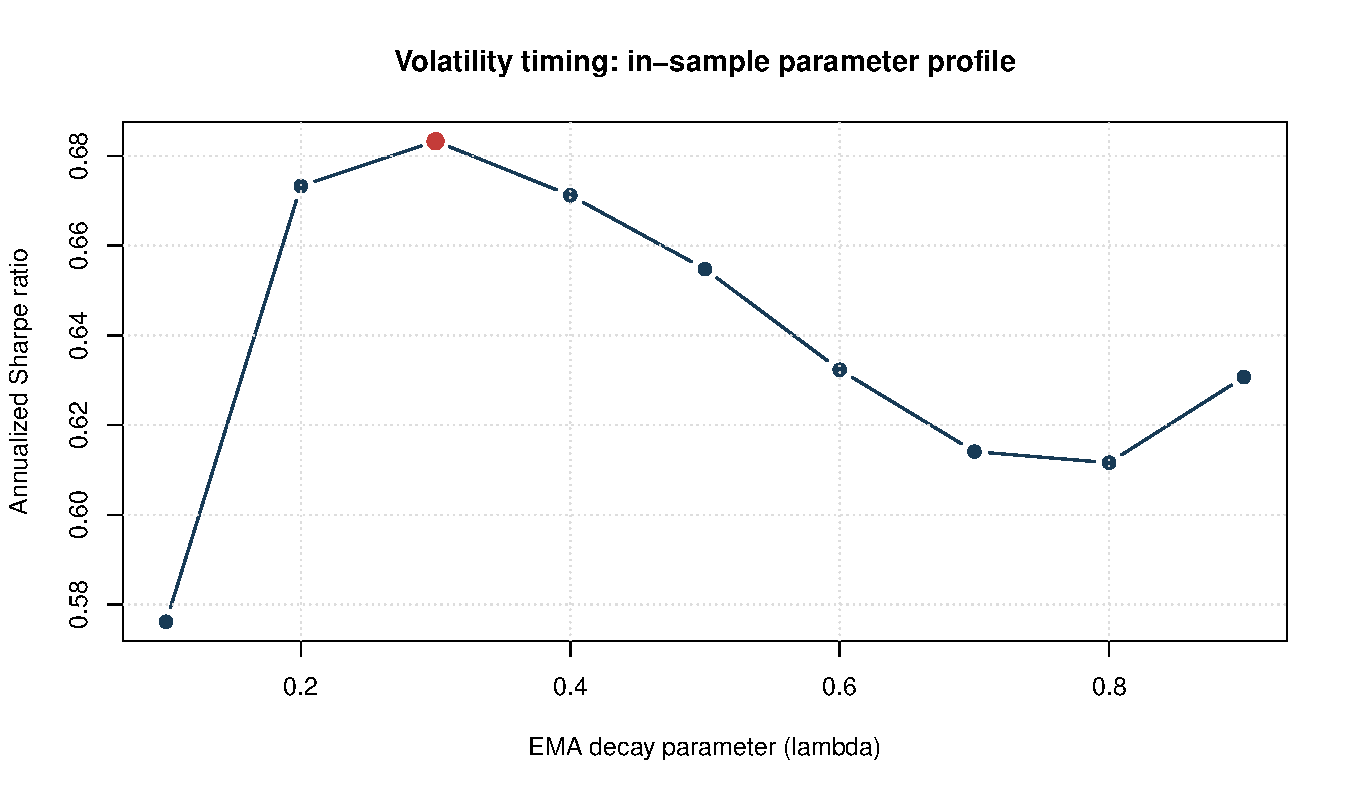
\includegraphics[width=0.86\linewidth]{figures/strat_voltiming_profile_ema.pdf}
\caption{Net strategy Sharpe ratio versus the EMA decay factor. Every point
uses the same complete historical SPY sample.}
\label{fig:lambdas}
\end{figure}

Smaller decay factors respond more quickly to recent returns and can
produce greater turnover. Larger factors smooth the volatility estimate
more heavily. Their Sharpe ratios reflect both this change in exposure and
the costs of adjusting it. The highest ratio is \HWBestSharpe{}, attained
at $\lambda=\HWBestLambda$. The maximum in Table~\ref{tab:lambdas} is an
in-sample parameter choice among nine alternatives; it is not evidence of
performance on an independent test sample.

\clearpage
\section{Part II: Hampel strategies for individual stocks}
\subsection{II.1: stock-level signals and Sharpe rankings}
An \texttt{lapply()} loop processes each stock separately. It removes missing
prices for that stock and omits a series with fewer than
$2\times\texttt{lookb}=6$ valid observations. Its PnL series retains the
stock's actual dates, including warmup observations with zero positions.
Removing missing prices means that consecutive valid observations may span
more than one trading date for an interrupted series.

Let $\ell_{t,j}=\log P_{t,j}$ be stock $j$'s log price. With a trailing
window of $L=3$ observations, define
\begin{align}
m_{t,j}&=\operatorname{median}
\{\ell_{t-L+1,j},\ldots,\ell_{t,j}\},\\
d_{t,j}&=1.4826\operatorname{median}
\{|\ell_{s,j}-m_{t,j}|:s=t-L+1,\ldots,t\},\\
z_{t,j}&=\begin{cases}
(\ell_{t,j}-m_{t,j})/d_{t,j},&d_{t,j}>0,\\
0,&d_{t,j}=0.
\end{cases}
\label{eq:hampel}
\end{align}
The factor $1.4826$ is the normal-consistency multiplier used by the
installed \texttt{HighFreq} nonparametric dispersion calculation. The
code calls \texttt{roll\_mean(..., method="nonparametric")} and
\texttt{roll\_var(..., method="nonparametric")} to obtain the trailing
median and scaled MAD. The first $L$ z-scores are set to zero.

The contrarian target position, with threshold one, is
\begin{equation}
h_{t,j}=\begin{cases}
-1,&z_{t,j}>1,\\
+1,&z_{t,j}<-1,\\
h_{t-1,j},&-1\leq z_{t,j}\leq1,
\end{cases}
\qquad h_{1,j}=0.
\label{eq:hampelpositions}
\end{equation}
Thus a price sufficiently above its trailing median triggers a short
position; a price sufficiently below it triggers a long position. A neutral
signal preserves the previous position. The code fills forward the target
positions, lags them by one observation, and calculates
\begin{equation}
r_{t,j}=\ell_{t,j}-\ell_{t-1,j},\qquad
\pi_{t,j}=h_{t-1,j}r_{t,j},
\label{eq:hampelpnl}
\end{equation}
using a zero first log-price difference. This retains zero warmup PnLs
without a look-ahead signal. No transaction costs are deducted in Part II,
as specified by the assignment's interpretation.

The resulting named list \texttt{pnls} stores a one-column \texttt{xts}
PnL series for each of the \HWEligibleStocks{} eligible stocks. Applying
Equation~\ref{eq:sharpe} to
each series and sorting in descending order produces the full-period
Sharpe ranking.

\smallinput{hampel_top10.tex}{Ten largest full-period stock-level Hampel
Sharpe ratios, calculated from the available stock universe. These ranks
use each stock's own valid observation history.}{tab:topten}

A high full-period Sharpe ratio here is a description of one stock's
historical strategy returns. The lengths and dates of stock histories
differ. These full-period rankings are not used to choose the out-of-sample
top-100 portfolio in Section~\ref{sec:top100}.

\subsection{II.2: the mean strategy and the NXPI example}
The stock PnLs are merged on the union of their dates. For each date $t$,
let $A_t$ contain stocks with an available PnL. The assignment's row mean
is
\begin{equation}
\overline\pi_t=\frac{1}{|A_t|}\sum_{j\in A_t}\pi_{t,j}.
\label{eq:meanportfolio}
\end{equation}
The code uses \texttt{rowMeans(..., na.rm=TRUE)} and preserves the date index
in a one-column \texttt{xts} series. Zero strategy positions remain valid
zero PnLs; unavailable stock observations are omitted from the average.
Consequently, the number and identity of stocks in the daily mean can
change over time. An all-missing row is marked missing rather than treated
as a zero return. The available count ranges from \HWMinAvailable{} to
\HWMaxAvailable{} stocks across the observed dates, out of 717 stocks
appearing somewhere in the input history.

\begin{figure}[H]\centering
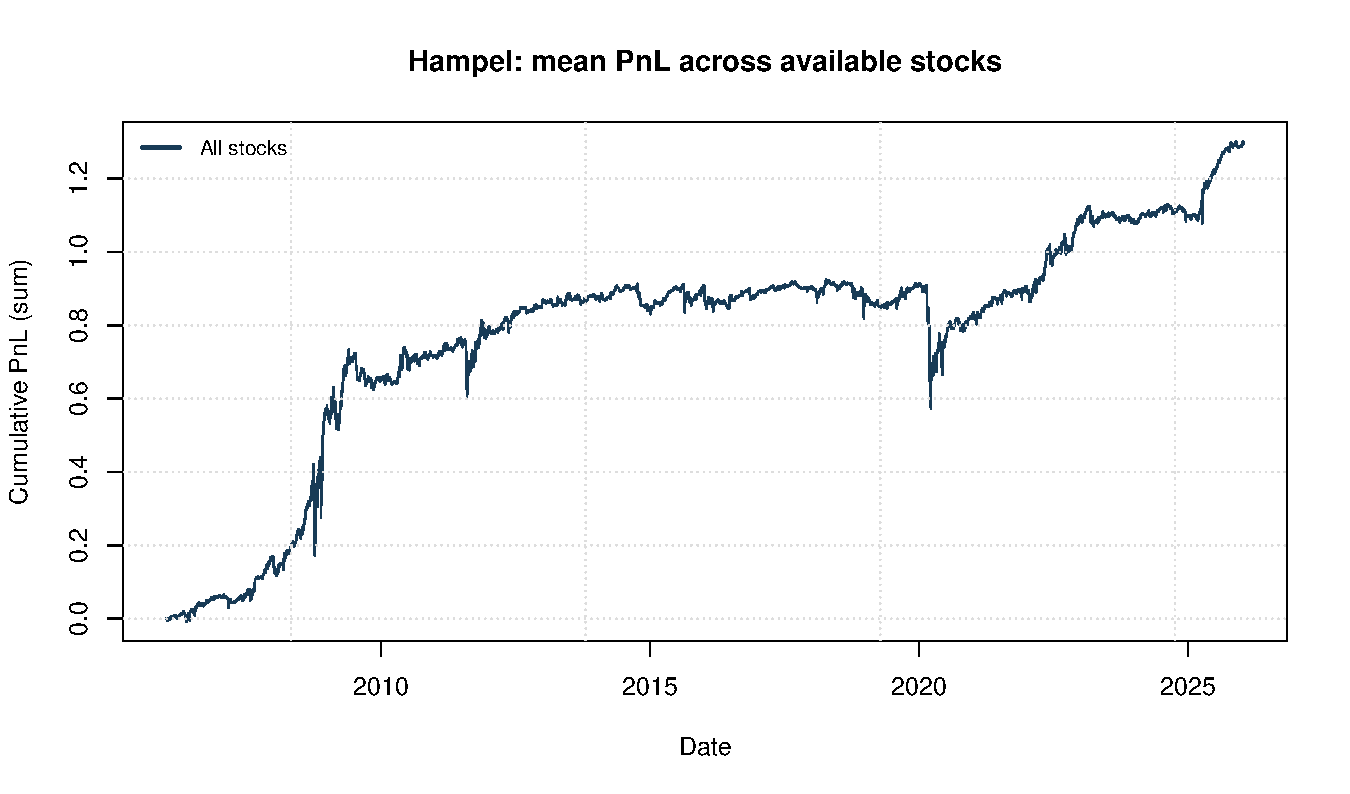
\includegraphics[width=0.94\linewidth]{figures/strat_hampel_mean.pdf}
\caption{Cumulative mean daily Hampel PnL across all available stock
strategies. The changing available-stock denominator follows
Equation~\ref{eq:meanportfolio}. No stock-strategy transaction costs are
deducted.}
\label{fig:hampelmean}
\end{figure}

The full-period Sharpe ratio of the all-stock mean PnL is
\HWAllFullSharpe{}. Averaging individual PnLs reduces variation arising
from imperfectly correlated stock strategies; this portfolio ratio is not
the arithmetic average of their individual Sharpe ratios.

The NXPI plot aligns its buy-and-hold daily log returns with the dates of
its Hampel strategy. Both cumulative curves begin with the same zero-return
convention. Their Sharpe ratios use the same overlapping observations, so
the comparison is not driven by unequal date samples.

\smallinput{nxpi_metrics.tex}{NXPI buy-and-hold and Hampel performance over
the same available dates. Part II excludes transaction costs.}{tab:nxpi}

NXPI's buy-and-hold Sharpe is \HWNxpiSharpe{}, compared with
\HWNxpiHampelSharpe{} for the Hampel strategy. This individual example
does not establish that the rule works equally well for other stocks.

\begin{figure}[H]\centering
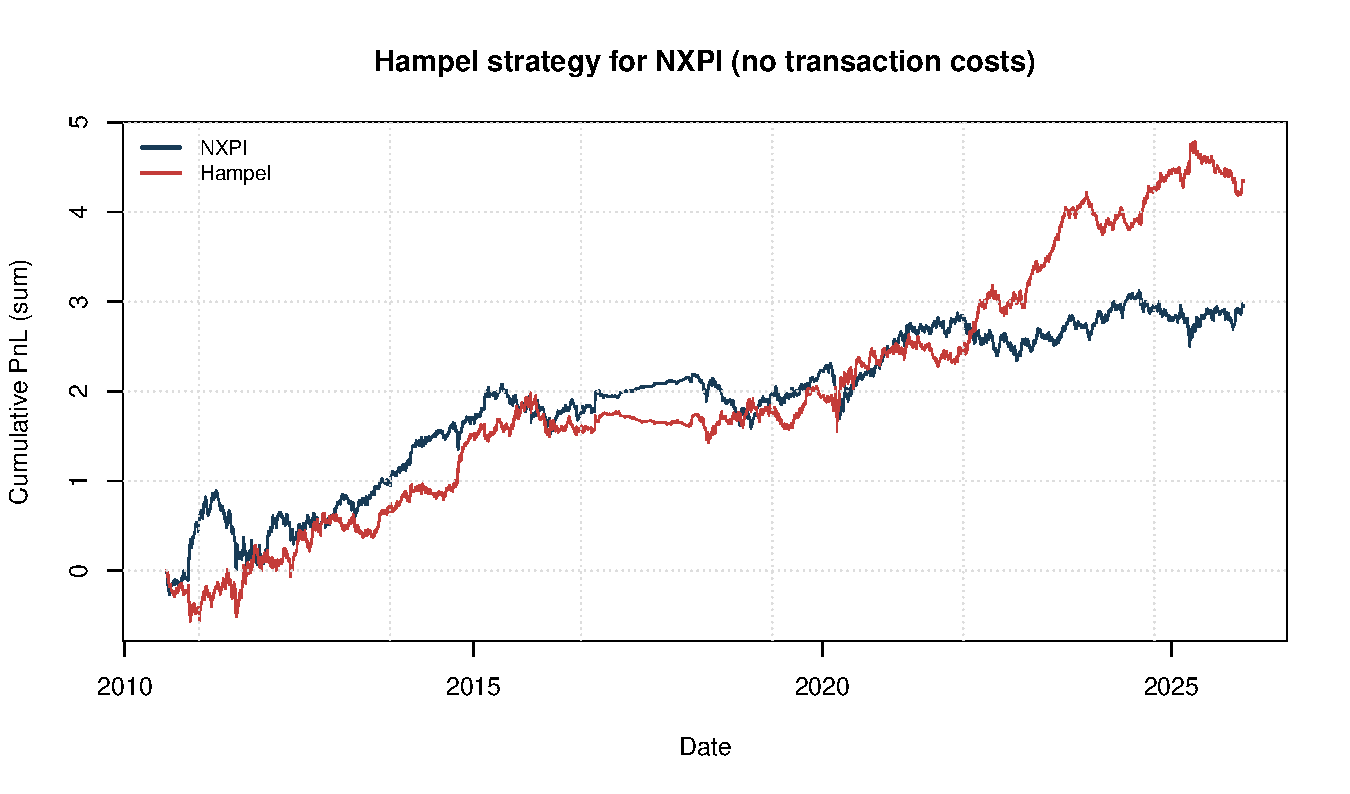
\includegraphics[width=0.94\linewidth]{figures/strat_hampel_single.pdf}
\caption{NXPI cumulative log returns and cumulative Hampel PnLs over NXPI's
available history. The delayed strategy can hold long or short positions.}
\label{fig:nxpi}
\end{figure}

The course asks for interactive \texttt{dygraphs}. The R submission writes
the requested interactive charts as HTML files alongside the corresponding
static report figures. The static plots allow the report to remain
self-contained when submitted as a PDF.

\subsection{II.3: in-sample and out-of-sample Sharpe persistence}
\label{sec:persistence}
The sample split is fixed at the end of 2016. The in-sample interval includes
dates through December 31, 2016; the out-of-sample interval begins January 1,
2017. Signals are generated sequentially on each stock's complete history,
so the first 2017 position can use the final observed information from 2016.
The split does not reset the trading position or recalculate past signals.

For each stock, the code calculates Sharpe ratios separately in the two
intervals and retains stocks with finite ratios in both. In particular,
stocks that began trading after 2016 cannot enter the comparison. Matching
by ticker places the same stocks in the same order in
\texttt{sharpis} and \texttt{sharpos}. The finite-ratio condition does not
impose a long minimum history within each interval. A stock observed for
only a short part of a subperiod can therefore have an unstable ratio and
appear as an extreme point. The scatterplot fits
\begin{equation}
\widehat{\mathrm{SR}}_{j,\mathrm{OS}}
=\widehat\alpha+\widehat\beta
\widehat{\mathrm{SR}}_{j,\mathrm{IS}}+e_j.
\label{eq:persistence}
\end{equation}

\smallinput{persistence.tex}{Cross-sectional relationship between stock
Hampel Sharpe ratios through 2016 and from 2017 onward. Only stocks with
finite ratios in both periods enter the regression.}{tab:persistence}

\begin{figure}[H]\centering
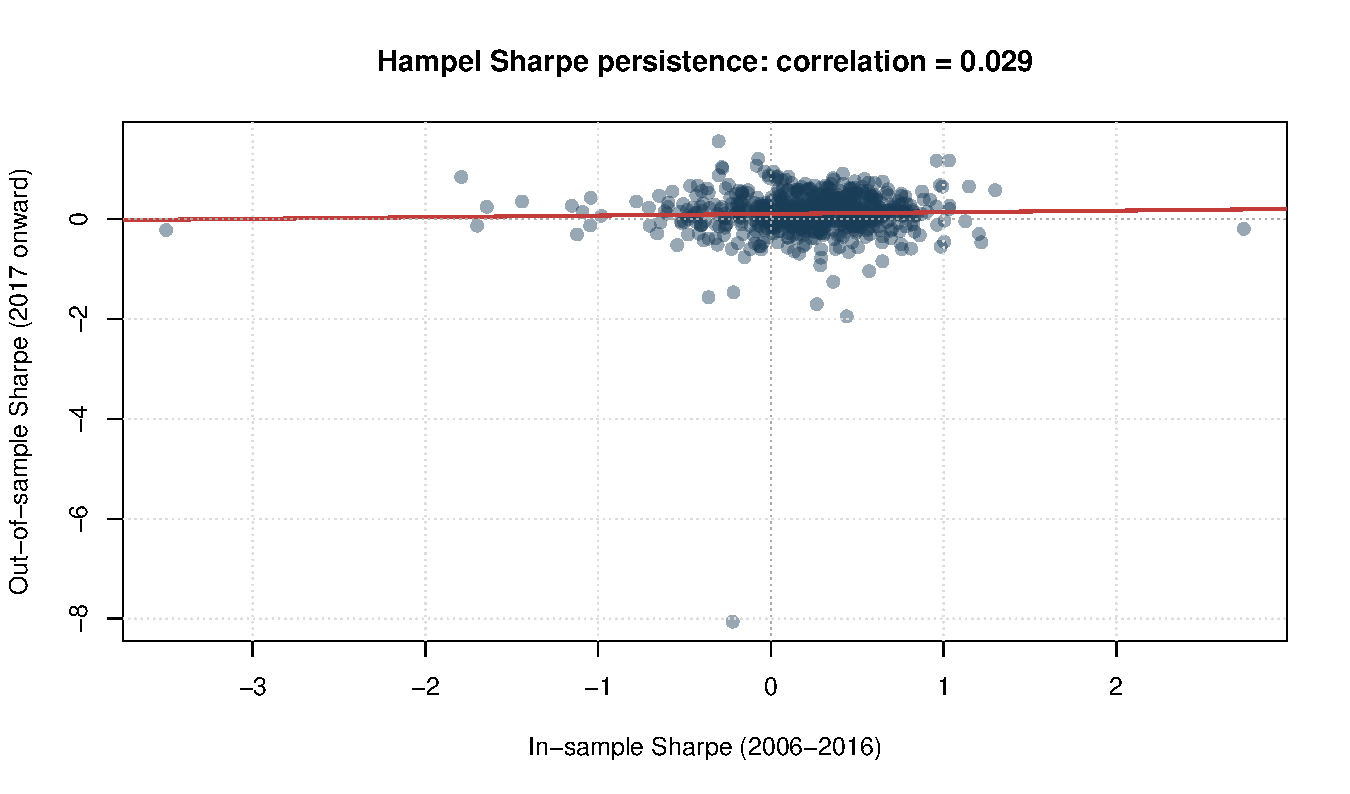
\includegraphics[width=0.88\linewidth]{figures/strat_hampel_scatter.pdf}
\caption{In-sample versus out-of-sample Hampel Sharpe ratios, with an
ordinary least-squares regression line. Each point represents the same
stock in the two periods.}
\label{fig:persistence}
\end{figure}

The fitted slope is \HWPersistenceSlope{}, the correlation is
\HWPersistenceCorrelation{}, and $R^2=\HWPersistenceRSquared$. The
conventional slope p-value is \HWPersistencePValue{}. The fitted
relationship explains very little of the out-of-sample variation, and the
available data provide little evidence of positive persistence. This
differs from the template's comment and reference figure, which use a
different stock dataset. A small positive fitted slope alone does not
justify a claim that large in-sample Sharpe ratios reliably predict large
later ratios.

Stocks are related through market and sector exposures, so a conventional
regression p-value should not be interpreted as if all stock observations
were independent experiments. The selected universe and unequal history
lengths are further limits on generalizing this comparison.

\subsection{II.4: the top-100 in-sample selection}
\label{sec:top100}
The selected tickers are the first 100 names after sorting
\emph{in-sample} Sharpe ratios in descending order. Their full-history PnL
series are then averaged using the same available-stock convention as
Equation~\ref{eq:meanportfolio}. No observation from 2017 onward is used to
rank the stocks, and later data availability is not used to filter the
in-sample selection. The plotted full history contains both the period used to
choose them and the subsequent evaluation period. The ticker selection is
fixed, while its daily average includes only selected stocks with data on
that date; a selected stock without later observations does not contribute
to the later mean. In this snapshot, four selected tickers---SIAL, HCBK,
SWY, and FDO---have no out-of-sample prices, leaving 96 selected stocks
that appear during the later period.

\begin{figure}[H]\centering
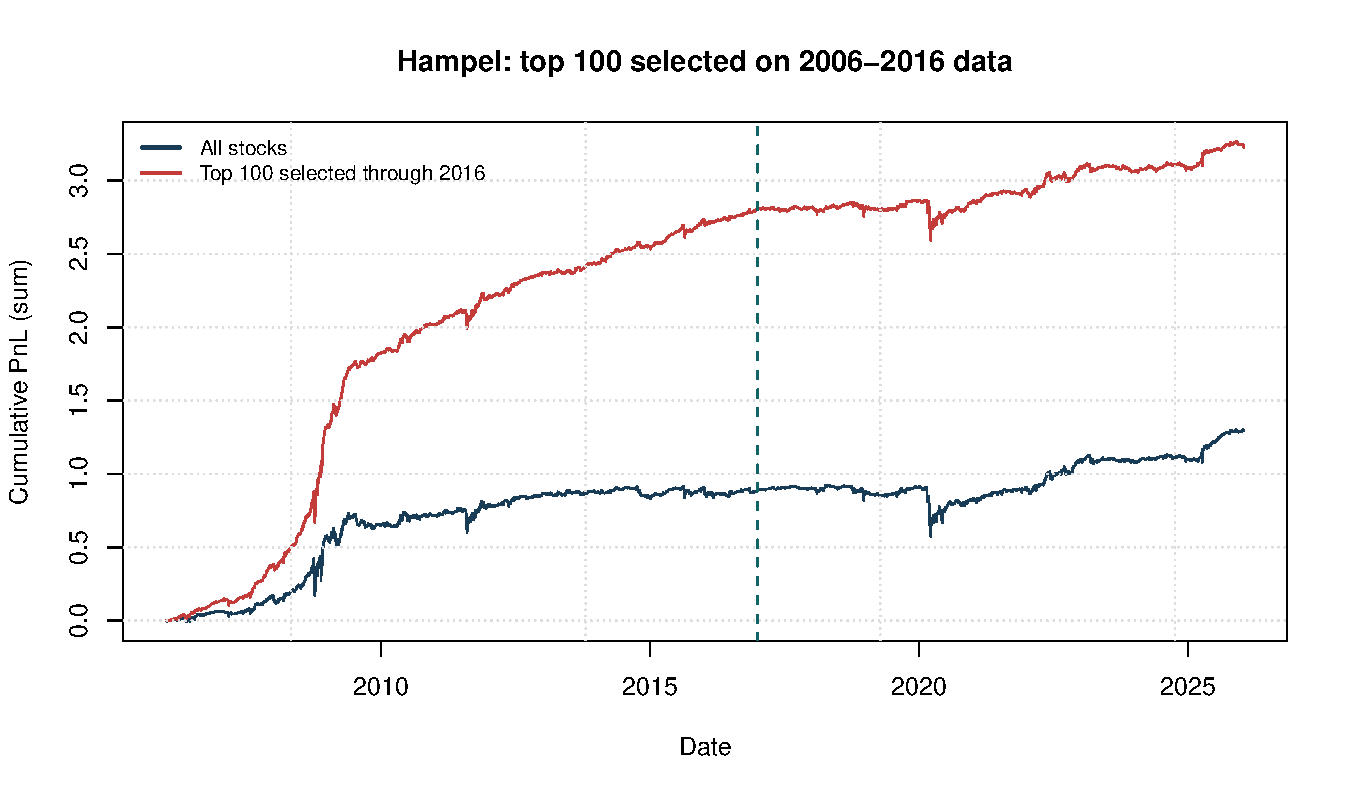
\includegraphics[width=0.94\linewidth]{figures/strat_hampel_top.pdf}
\caption{Cumulative mean Hampel PnL for the 100 stocks with the highest
in-sample Sharpe ratios. The vertical split marks the start of 2017. The
earlier segment is selected in sample; the later segment evaluates the
available members of that fixed ticker selection.}
\label{fig:top100}
\end{figure}

\wideinput{portfolio_metrics.tex}{Mean-portfolio performance for all stocks
and for the top 100 selected using only data through 2016. The separate
out-of-sample rows evaluate dates from 2017 onward. Cumulative PnL is a sum
of daily strategy PnLs.}{tab:portfolios}

The top-100 mean portfolio's annualized Sharpe falls from
\HWTopISSharpe{} in sample to \HWTopOOSSharpe{} out of sample.
Selection favors stocks with unusually good in-sample realizations, so the
early top-100 curve is optimistically selected by construction. The later
rows in Table~\ref{tab:portfolios} show that the striking early performance
does not carry forward at a comparable risk-adjusted level. These results
still use the course's supplied stock
universe and omit spread, slippage, stock-borrow, and financing costs.
Short positions and frequent position reversals can make these omissions
material. Historical membership and delisted-stock coverage are not
established by the input file, so the analysis cannot exclude survivorship
or universe-selection bias.

\section{Numerical checks and deliverables}
The verification record reports 63 passing checks. It checks calculations
using independent reconstructions
of the position delays, turnover costs, volatility scaling, and performance
ratios. It also checks the parallel parameter sweep against a serial
calculation and verifies the Hampel positions, date alignment, sample split,
and restriction of top-100 ranking inputs to the first period.

The completed R file implements all six tasks, with a labeled section for
each question. The original \texttt{FRE7241\_hw2.R} is retained separately.
The repository stores the inputs and the derived numerical
tables so that the figures and report can be regenerated. The report's
tables are exported from computed results instead of transcribed from the
template. The README gives the package setup, R execution, and LaTeX build
commands. The principal submission artifacts are:
\begin{itemize}
\item \texttt{Panagiotis\_Housos\_hw2.R}, the completed R assignment;
\item \texttt{report/Panagiotis\_Housos\_HW2\_Report.pdf}, this report;
\item the public repository at
\url{https://github.com/ph2606/fre7241-homework-02}.
\end{itemize}

The parameter sweep is in sample, Part I's volatility scale uses the
full sample, and its two-return startup has the initialization exception
described above. Part II's time split gives a later comparison period for
stock selection, but costs and historical universe membership remain limitations.
These are historical simulations rather than validated investment
recommendations.

\begin{thebibliography}{9}
\raggedright
\bibitem{univariate} J. Pawlowski. \emph{Univariate Investment Strategies},
FRE7241 course slides, January 20, 2026, especially the trailing volatility
example on slide 27 and the Hampel filter examples on slides 88--90.
\bibitem{app} J. Pawlowski. \texttt{app\_hampel\_simple.R}, supplied course
Shiny example under \texttt{05\_Code\_Examples/Shiny\_Apps/}. The submitted
assignment follows the lecture's log-price formulation.
\bibitem{assignment} J. Pawlowski. \texttt{FRE7241\_hw2.R} and six supplied
reference figures. Homework 2, due November 10, 2026, at 6 p.m.
\bibitem{packages} Installed \texttt{rutils} and \texttt{HighFreq}
implementations. Exact package versions and source information accompany
the submission under \texttt{reproducibility/}.
\end{thebibliography}

\clearpage
\appendix
\section{Complete submitted R code}
\label{app:code}
The submission labels and completes all six questions. The original
assignment and its illustrative output comments are supplied separately
as \texttt{FRE7241\_hw2.R}. Actual computed outputs use the frozen inputs
documented in Section~\ref{sec:data}.
\lstinputlisting{../Panagiotis_Housos_hw2.R}

\clearpage
\section{Independent verification record}
\label{app:verification}
\lstinputlisting[language={},numbers=none,basicstyle=\ttfamily\footnotesize,
  xleftmargin=0pt,framexleftmargin=0pt]{../hw2_results/verification.txt}
\end{document}
